\documentclass[11pt,a4paper]{article}
\usepackage[utf8]{inputenc}
\usepackage[T1]{fontenc}
\usepackage{mathptmx}
\usepackage[margin=0.9in]{geometry}
\usepackage{graphicx}
\usepackage{booktabs}
\usepackage{array}
\usepackage{amsmath}
\usepackage{hyperref}
\usepackage{listings}
\usepackage{xcolor}
\usepackage{float}

\lstset{
  language=Python,
  basicstyle=\ttfamily\small,
  breaklines=true,
  frame=single,
  backgroundcolor=\color{gray!8}
}

\begin{document}

% Page 1: Title Page
\begin{titlepage}
\centering
\vspace*{1.5cm}

{\large\bfseries Thapar Institute of Engineering and Technology, Patiala\par}
{\large Department of Computer Science and Engineering\par}

\vspace{2.2cm}
{\Huge\bfseries Hit Song Predictor\par}
\vspace{0.3cm}
{\large\itshape Predicting Chart Success from Audio Features\par}

\vspace{1.8cm}
{\large\textbf{Subject:} Machine Learning Lab (UML501)\par}
\vspace{0.2cm}
{\large\textbf{Group:} 3Q24\par}

\vspace{1.4cm}
{\large\textbf{Submitted By}\par}
\vspace{0.2cm}
{\large Shivansh Sahu -- Roll No. 1024170249\par}
{\large Kaif Ahmad -- Roll No. 1024170255\par}

\vspace{1.4cm}
{\large\textbf{Submitted To}\par}
\vspace{0.2cm}
{\large Mr. Shiwam Kumar\par}

\vspace{1.4cm}
{\large\textbf{Academic Session:} 2026 - 2027\par}

\vfill
\end{titlepage}

\section*{2. Abstract}
Record labels decide which songs to fund and promote long before anyone knows whether they will succeed, and these decisions often rely on instinct. Streaming platforms, however, already measure every track automatically through audio features such as tempo, energy, danceability and loudness. This project asks a simple, testable question: can a song's measurable properties predict whether it will appear on the Billboard Year-End Hot 100?

We treat the problem as a supervised binary classification task. The dataset combines the Billboard Year-End Hot 100 (2000--2023) with Spotify audio features and contains 7,403 songs, of which only 673 (9.1\%) charted. Because of this strong class imbalance, accuracy alone is misleading, so we report precision, recall, F1-score and ROC-AUC, and use stratified, artist-disjoint train/test splits to prevent leakage. Seven model configurations were trained on identical data: Logistic Regression, Decision Tree (Gini), Decision Tree (Entropy), Random Forest, Naive Bayes, K-Nearest Neighbours and SVM (linear and RBF). Hyperparameters were tuned with stratified cross-validation, and the final model was chosen by weighing interpretability against performance.

Random Forest feature importance shows that genre is the most influential input, followed by loudness and instrumentalness. A threshold study shows how predictions change with business priorities. The best model reached $F_1 = 0.5204$, $\text{ROC-AUC} = 0.929$ on the held-out test set. A form-based demo returns a chart/no-chart label with a probability score.

\section*{3. Introduction}
\subsection*{3.1 Problem Domain}
The music industry produces an enormous number of tracks every year, but only a small fraction reach the Billboard Hot 100. Artists-and-repertoire (A\&R) teams must choose which songs to promote with limited budgets and incomplete information. Machine learning offers a data-driven way to support this choice by learning patterns from songs that charted in the past.

\subsection*{3.2 Motivation}
We chose this project because it uses objective data on both sides: every input feature is computed by software (no human labelling or taste involved) and the label is a matter of public record (a song either charted or it did not). It also lets us apply almost all the classification algorithms studied in the course on one realistic dataset, and it exposes a common real-world difficulty: severe class imbalance.

\subsection*{3.3 Importance}
An accurate and explainable model can help labels prioritise promotion, help artists understand which sound properties are associated with charting, and test industry folklore such as ``upbeat songs chart better'' or ``songs are getting shorter'' with evidence instead of anecdotes.

\subsection*{3.4 Objectives}
\begin{itemize}
  \item Build and compare seven classification configurations on the same data split.
  \item Handle class imbalance correctly and evaluate with metrics suited to it.
  \item Identify which audio features most influence chart success.
  \item Study how the decision threshold changes predictions under different business priorities.
  \item Justify a final model by trading off interpretability and performance, and deploy it as a simple prediction demo.
\end{itemize}

\section*{4. Problem Statement}
Given a song's audio features and metadata, predict whether it will appear on the Billboard Hot 100 or fail to chart. The input is a vector of ten attributes (tempo, energy, danceability, valence, loudness, acousticness, instrumentalness, speechiness, duration and genre). The output is a binary label ($1 =$ charted, $0 =$ did not chart) together with a probability score for every prediction.

The purpose of the proposed solution is to give decision-makers a quantified, explainable estimate of chart potential. The expected outcome is a trained classifier, a full model comparison, a ranked list of influential features and an argued choice of final model, rather than a simple statement of which model has the highest accuracy.

\section*{5. Literature Review}
\textbf{Existing approaches.} Earlier studies on hit prediction use audio descriptors from streaming platforms and train standard classifiers to separate hits from non-hits. Middlebrook and Sheik [4] used Spotify data to predict Billboard hits and compared several machine-learning models, showing that audio features carry measurable, though limited, predictive signal.

\textbf{Previously developed solutions.} Practical solutions generally combine Spotify audio features with chart history from Billboard, which is the same data strategy used here. Public datasets such as the Billboard Hot-100 (2000--2023) data with features [1] make this approach reproducible.

\textbf{Limitations of existing approaches.} Many reported results emphasise accuracy even though hits are rare, which can hide poor recall. Random train/test splits can also place songs of the same artist in both sets, so the model may partly recognise the artist rather than the sound. Finally, a song's success depends on factors that audio features cannot capture, such as marketing, artist popularity and release timing.

\textbf{How this project addresses them.} We use imbalance-aware metrics, stratified and artist-disjoint splits, a fair comparison on identical data, explainability through feature importance, and a threshold study linked to business cost.

\section*{6. Dataset Description}
\subsection*{6.1 Source and Size}
The data combines the Billboard Year-End Hot 100 with the Spotify 114k Tracks dataset, using the Kaggle dataset ``Billboard Hot-100 [2000--2023] Data with Features'' by Biswas [1]. It contains \textbf{7,403 songs}, of which \textbf{673 (9.1\%)} charted. Spotify shut down its live Audio Features API in November 2024 [3], so new applications can no longer collect this data directly; we therefore use an existing pre-scraped dataset with identical feature columns.

\begin{table}[H]
\centering
\caption{Input and output attributes}
\begin{tabular}{llp{8cm}}
\toprule
\textbf{Attribute} & \textbf{Type} & \textbf{Description} \\
\midrule
Tempo & Numeric & Estimated speed of the track in beats per minute (BPM) \\
Energy & Numeric (0--1) & Perceived intensity and activity \\
Danceability & Numeric (0--1) & How suitable the track is for dancing \\
Valence & Numeric (0--1) & Musical positivity (happy vs sad mood) \\
Loudness & Numeric (dB) & Overall loudness of the track \\
Acousticness & Numeric (0--1) & Confidence that the track is acoustic \\
Instrumentalness & Numeric (0--1) & Likelihood the track has no vocals \\
Speechiness & Numeric (0--1) & Presence of spoken words \\
Duration & Numeric & Length of the track (seconds) \\
Genre & Categorical & Genre tag of the track \\
charted (target) & Binary & 1 if the song appears in a Billboard Year-End Hot 100 (2000--2023), else 0 \\
\bottomrule
\end{tabular}
\end{table}

\subsection*{6.2 Sample Data}
\begin{table}[H]
\centering
\caption{Sample records from the dataset (\texttt{df.head(5)})}
\scriptsize
\begin{tabular}{rrrrrrrrrll}
\toprule
tempo & energy & dance. & val. & loud. & acoust. & instr. & speech. & dur\_s & genre & charted \\
\midrule
90.15 & 0.298 & 0.653 & 0.812 & -15.50 & 0.044 & 0.000 & 0.439 & 170.95 & kids & 0 \\
131.41 & 0.005 & 0.205 & 0.033 & -35.52 & 0.988 & 0.941 & 0.094 & 154.01 & sleep & 0 \\
100.10 & 0.960 & 0.333 & 0.566 & -8.92 & 0.000 & 0.032 & 0.077 & 256.11 & heavy-metal & 0 \\
97.29 & 0.868 & 0.398 & 0.149 & -16.00 & 0.276 & 0.770 & 0.051 & 93.45 & sleep & 0 \\
111.00 & 0.593 & 0.745 & 0.170 & -6.35 & 0.005 & 0.000 & 0.052 & 212.03 & electro & 1 \\
\bottomrule
\end{tabular}
\end{table}

\subsection*{6.3 Challenges and Biases in the Dataset}
\begin{itemize}
  \item \textbf{Class imbalance.} Only 9.1\% of songs charted (Figure 1). A model that always predicts ``never charts'' would be about 91\% accurate yet useless. We addressed this by using precision, recall, F1 and ROC-AUC as the main metrics and stratified splits that preserve the class ratio.
  \item \textbf{Artist leakage.} Songs by the same artist share a recognisable sound. A random split could place them in both train and test sets and inflate results, so the 80/20 split is stratified and artist-disjoint.
  \item \textbf{Label definition.} The target uses the Year-End Hot 100 only, so a song that charted weekly but missed the year-end list is labelled 0. This is a known simplification.
  \item \textbf{Distribution and time bias.} The modelling dataset's class ratio may differ from the natural ratio of all released songs, and audio trends (for example loudness) change between 2000 and 2023. Results should therefore be read as indicative, not as a guarantee for future songs.
  \item \textbf{Data availability.} Because the Spotify API is closed to new apps, we relied on a pre-scraped dataset, which limits adding new songs.
\end{itemize}

\begin{figure}[H]
\centering
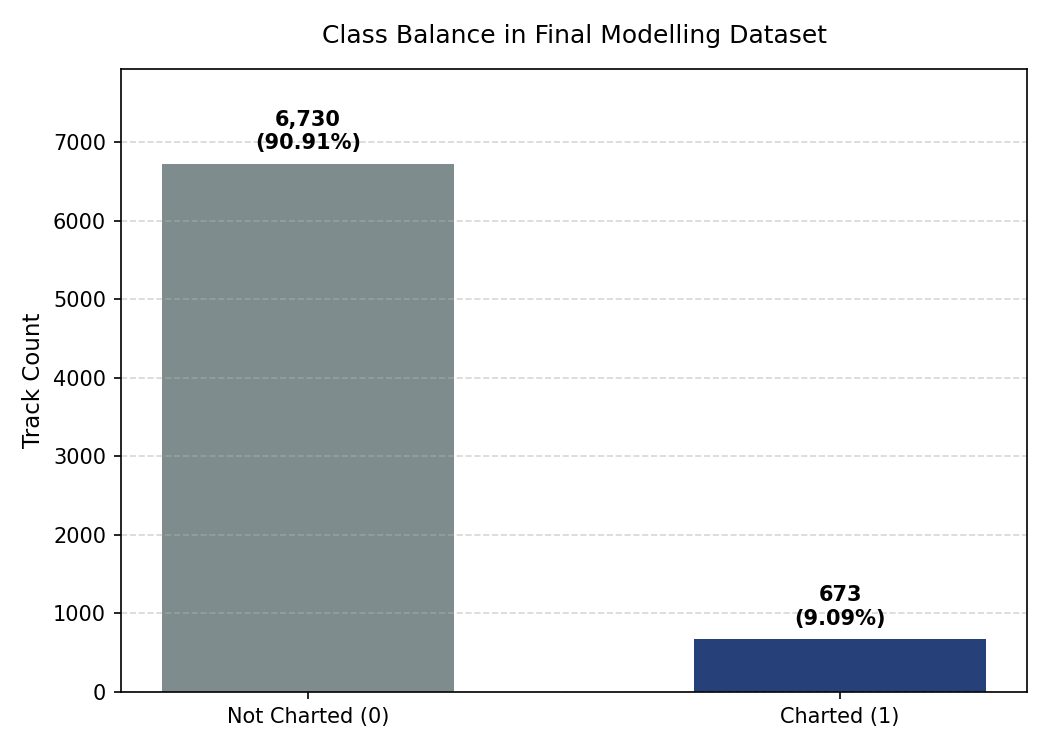
\includegraphics[width=0.68\textwidth]{figures/class_balance_modeling.png}
\caption{Class distribution of the 7,403 songs}
\end{figure}

\section*{7. Methodology}
The project follows six stages: pre-processing, exploratory analysis, model training, evaluation, analysis and deployment (Figure 2). All models use the same split so that the comparison is fair.

\begin{figure}[H]
\centering
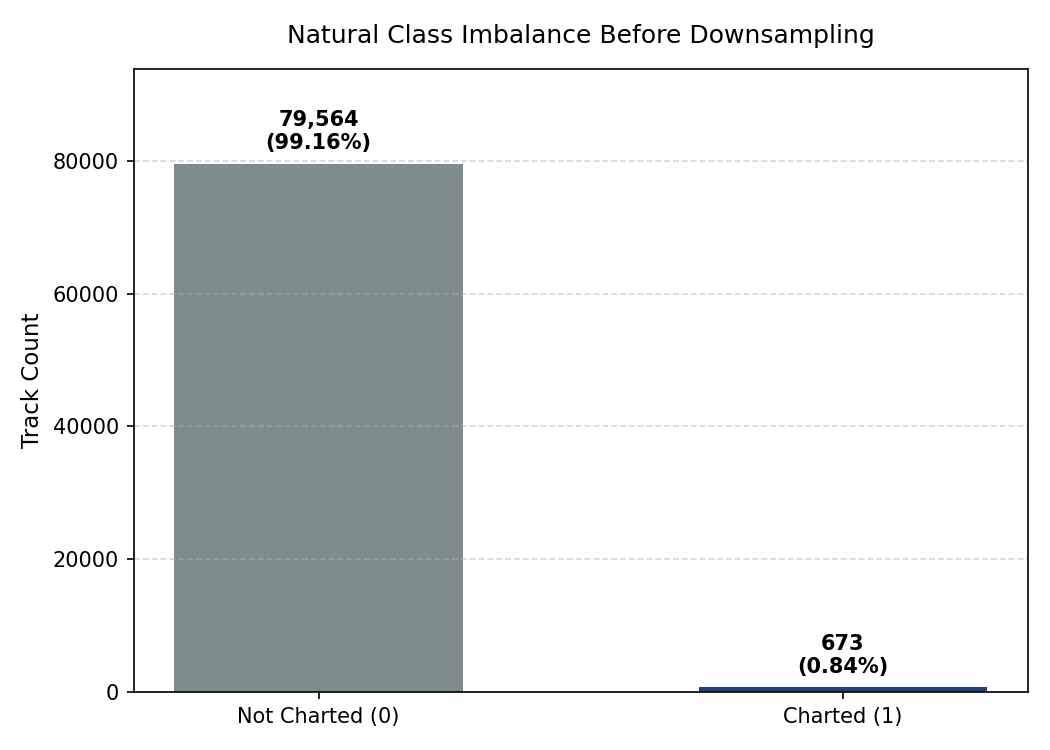
\includegraphics[width=0.68\textwidth]{figures/class_balance_natural.png}
\caption{Natural class distribution vs. modelling workflow}
\end{figure}

\subsection*{7.1 Data Collection}
Chart labels come from the Billboard Year-End Hot 100 (2000--2023) and audio features from Spotify's audio analysis, merged into one table with ten input features and one target [1].

\subsection*{7.2 Data Pre-processing and Feature Engineering}
\begin{itemize}
  \item \textbf{Missing values:} numeric gaps were imputed (median is robust to outliers) and rows missing a target were removed.
  \item \textbf{Duplicates:} repeated tracks were removed so the same song cannot appear in both train and test sets.
  \item \textbf{Encoding:} the categorical Genre was converted to numeric form (one-hot encoding) so that distance- and margin-based models can use it.
  \item \textbf{Scaling:} numeric features were standardised. This matters for KNN and SVM, which depend on distances and margins, and for the convergence of Logistic Regression. Tree-based models do not need scaling.
  \item \textbf{Feature engineering:} the main engineering step was aggregating the one-hot genre columns back into a single ``Genre'' importance when interpreting the Random Forest, so that genre is not split across many small bars. Additional derived features included converting \texttt{duration\_ms} to \texttt{duration\_sec} and normalising \texttt{primary\_artist} names for artist-disjoint grouping.
  \item \textbf{Splitting:} an 80/20 stratified, artist-disjoint split; the test set is kept untouched until the final evaluation. Scalers and encoders are fit on the training data only, to avoid leakage.
\end{itemize}

\subsection*{7.3 Exploratory Data Analysis and Visualisation}
EDA used histograms of each feature, scatter plots of feature pairs, box plots by class and a correlation heatmap. The main insights were:
\begin{itemize}
  \item The target is highly imbalanced (Figure 1), which shaped the whole evaluation strategy.
  \item Genre carries the largest share of predictive information (Figure 3), meaning where a song sits in the genre landscape matters more than any single audio measure.
  \item Loudness and instrumentalness come next, while tempo and speechiness contribute least in the Random Forest.
  \item Several audio features overlap in what they measure: energy--loudness ($r = +0.748$), energy--acousticness ($r = -0.720$), loudness--acousticness ($r = -0.575$), and danceability--valence ($r = +0.480$). This breaks the independence assumption of Naive Bayes and is a reason to expect it to perform weakest.
  \item Feature distributions differ between charted and non-charted songs only slightly for most features, which indicates the task is hard and that high accuracy should not be expected.
\end{itemize}

\begin{figure}[H]
\centering
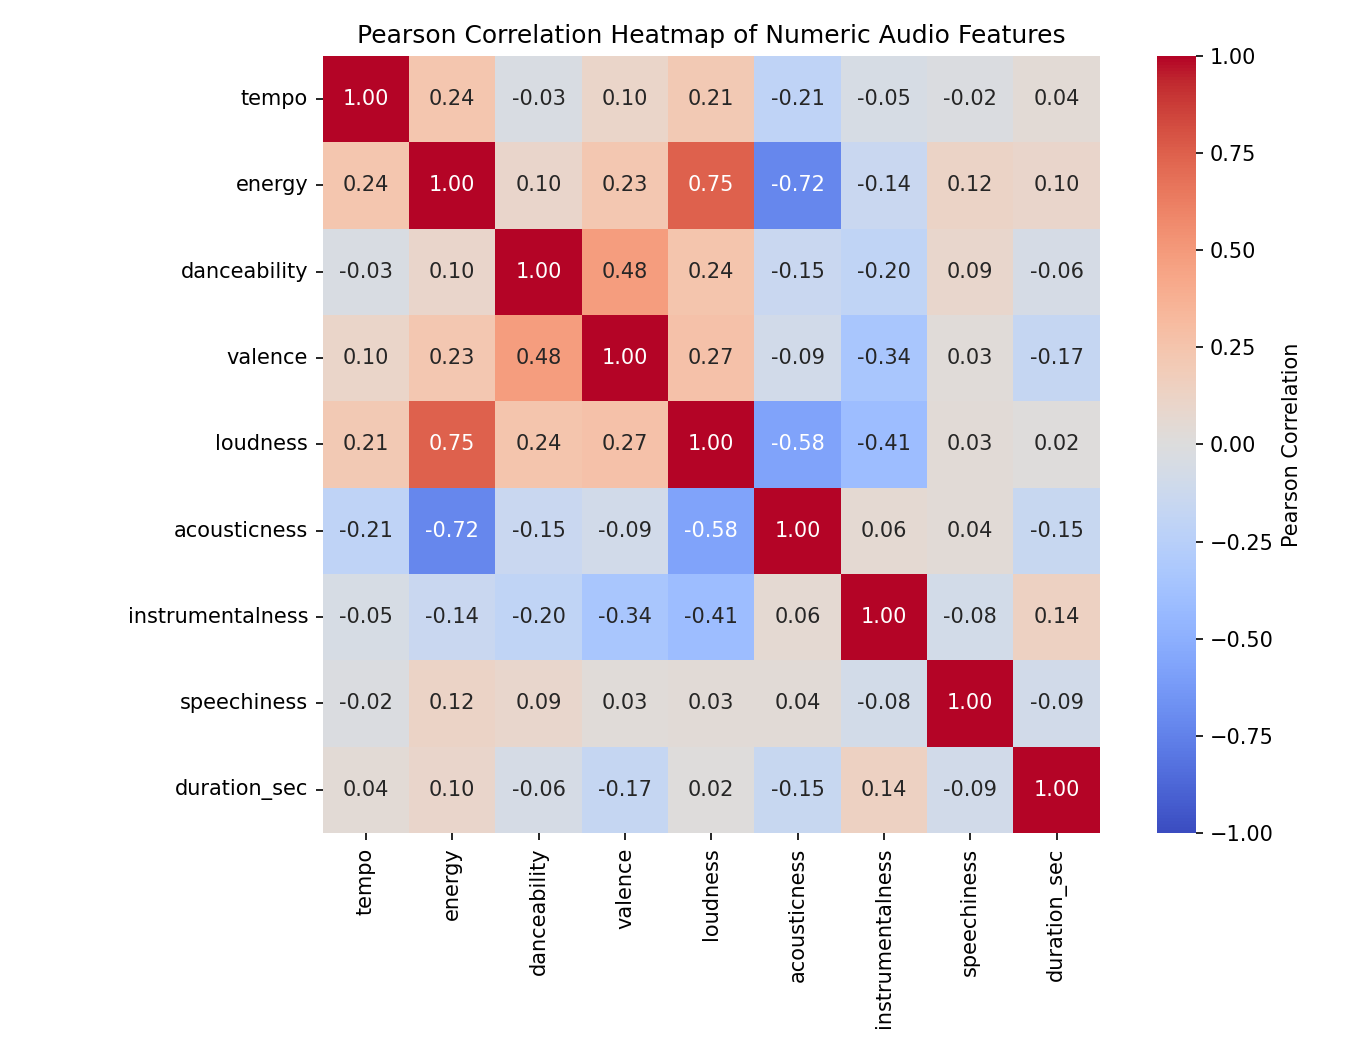
\includegraphics[width=0.72\textwidth]{figures/correlation_heatmap.png}
\caption{Exploratory data analysis correlation heatmap}
\end{figure}

\subsection*{7.4 Feature Selection}
All ten features were retained because the set is small and every feature is meaningful. Instead of removing features, we used Random Forest importance (Figure 3) to explain which features matter.

\begin{figure}[H]
\centering
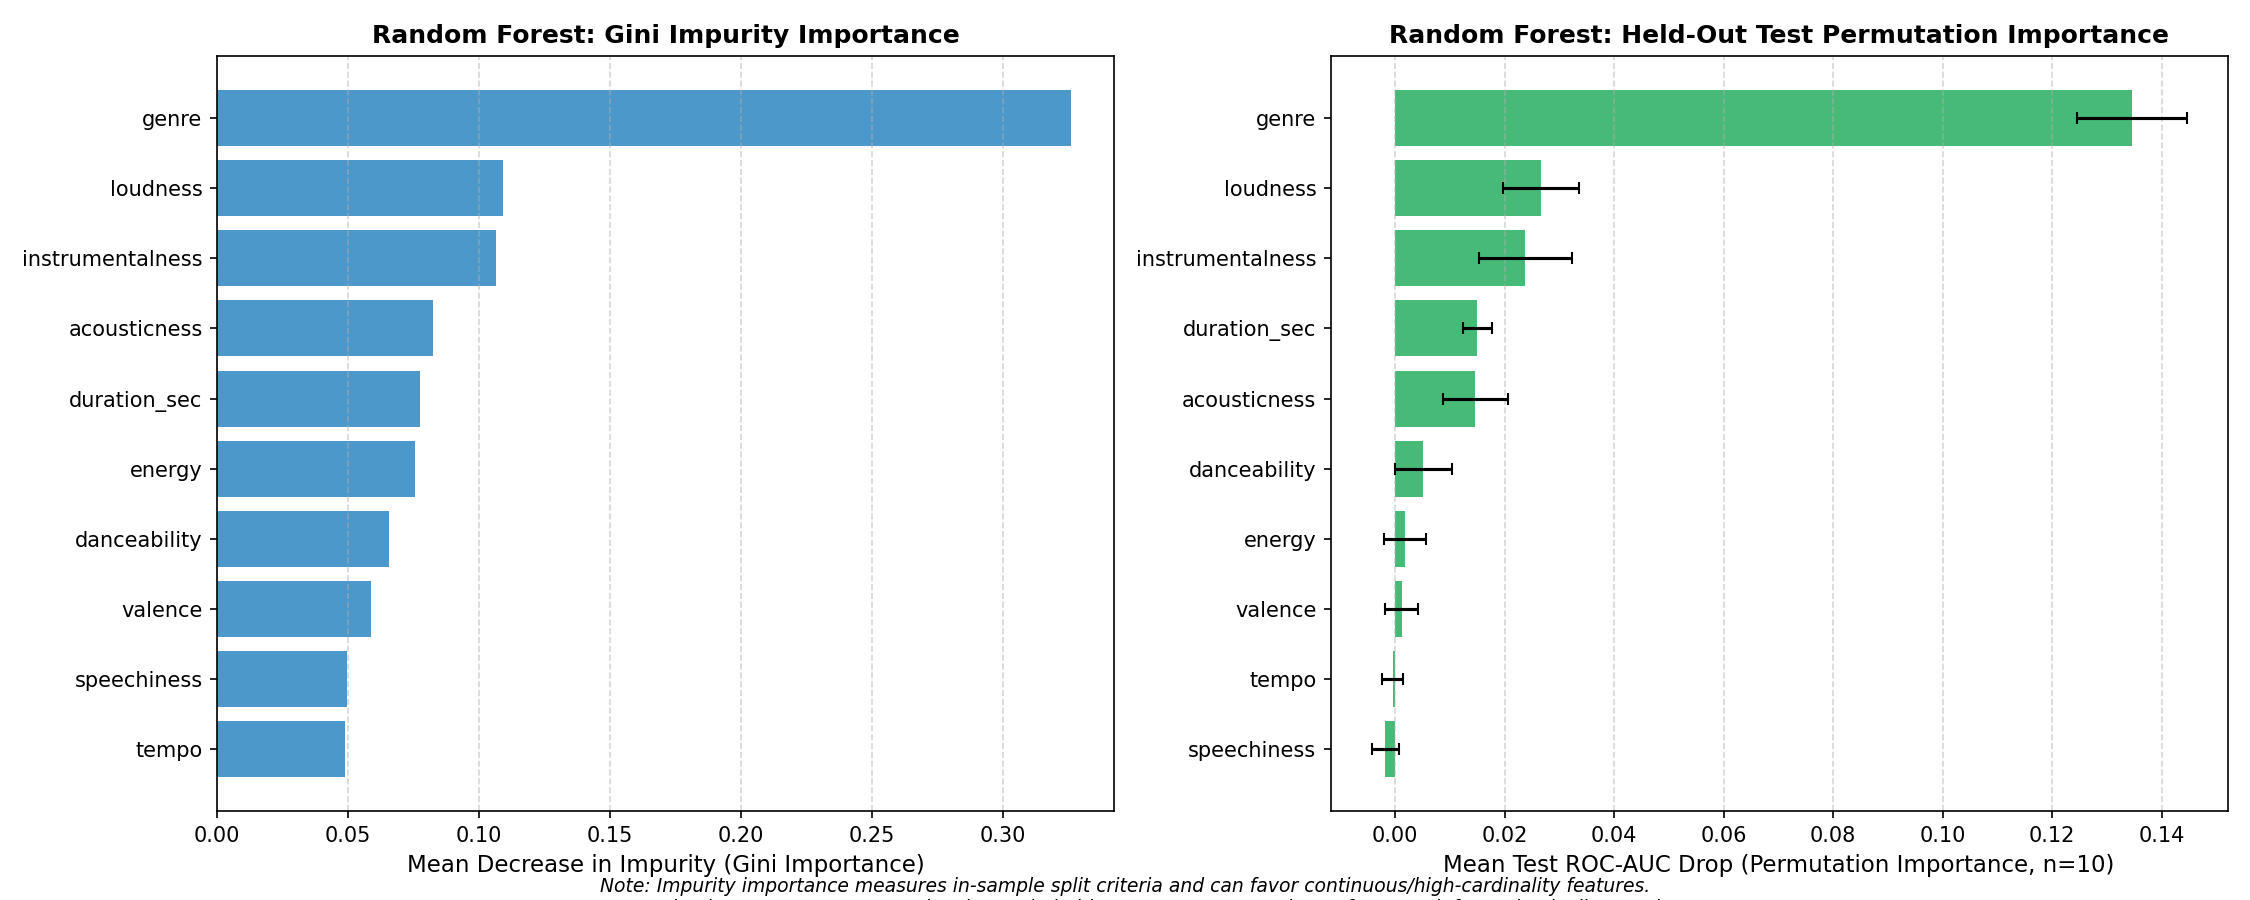
\includegraphics[width=0.82\textwidth]{figures/feature_importance_rf.png}
\caption{Random Forest feature importance (Gini, genre aggregated) vs. permutation importance}
\end{figure}

\subsection*{7.5 Machine Learning Algorithms Used}
\begin{table}[H]
\centering
\caption{Models used and their role (mapped to course topics)}
\begin{tabular}{lp{6.5cm}p{3.8cm}}
\toprule
\textbf{Model} & \textbf{Why it was included} & \textbf{Course topic} \\
\midrule
Logistic Regression & Interpretable coefficients show which features raise or lower chart odds; gives probabilities & Logistic regression, regularisation \\
Decision Tree (Gini) & Simple, readable splits on the purest thresholds & Decision trees (CART) \\
Decision Tree (Entropy) & Tests whether the split criterion changes the top features & Decision trees (information gain) \\
Random Forest & Ensemble that captures feature interactions a single tree misses & Ensembles, bagging \\
Naive Bayes & Fast baseline; assumes feature independence, which audio data breaks & Na\"ive Bayes \\
K-Nearest Neighbours & Votes among the $k$ most similar songs in scaled feature space & KNN \\
SVM (linear and RBF) & Maximum-margin boundary; tests linear separability & SVM \\
K-Means (bonus) & Unsupervised check for natural sound clusters, ignoring the label & Clustering / unsupervised learning \\
\bottomrule
\end{tabular}
\end{table}

\subsection*{7.6 Model Training and Testing}
Each model was trained on the training set and evaluated on the same held-out test set. Hyperparameters were chosen using stratified k-fold cross-validation on the training data only, so the test set never influenced model choice.

\section*{8. Implementation}
\subsection*{8.1 Platform and Libraries}
The project was implemented in \textbf{Python 3.11+} using \textbf{Visual Studio Code} (standalone modular scripts in \texttt{src/} plus FastAPI/Uvicorn). Libraries: \textbf{pandas} and \textbf{NumPy} for data handling, \textbf{Matplotlib} and \textbf{Seaborn} for visualisation, and \textbf{scikit-learn} for pre-processing, models, cross-validation and metrics [5].

\subsection*{8.2 Implementation Steps}
\begin{itemize}
  \item Load the merged dataset and inspect shape, types, missing values and duplicates.
  \item Clean the data, encode Genre, create the artist-disjoint stratified split, then fit the scaler on training data.
  \item Perform EDA and plot the class distribution and correlation heatmap.
  \item Train the seven configurations on the same split and tune hyperparameters with cross-validation.
  \item Evaluate every model with six metrics, a confusion matrix and overlaid ROC curves.
  \item Compute feature importance, run the threshold study and K-Means clustering.
  \item Save the chosen model and build the prediction demo.
\end{itemize}

\subsection*{8.3 Representative Code Snippet}
\begin{lstlisting}
from sklearn.pipeline import Pipeline
from sklearn.compose import ColumnTransformer
from sklearn.preprocessing import StandardScaler, OneHotEncoder
from sklearn.linear_model import LogisticRegression
from sklearn.model_selection import StratifiedGroupKFold, GridSearchCV

pre = ColumnTransformer([("num", StandardScaler(), NUMERIC_FEATURES),
                         ("cat", OneHotEncoder(handle_unknown="ignore", drop="first"), ["genre"])])
model = Pipeline([("preprocessor", pre),
                  ("model", LogisticRegression(max_iter=2000, class_weight="balanced", random_state=42))])
cv = StratifiedGroupKFold(n_splits=5, shuffle=True, random_state=42)
grid = GridSearchCV(model, {"model__C": [0.01, 0.1, 1.0, 10.0]}, cv=cv, scoring="roc_auc")
grid.fit(X_train, y_train, groups=groups_train)
\end{lstlisting}

\begin{figure}[H]
\centering
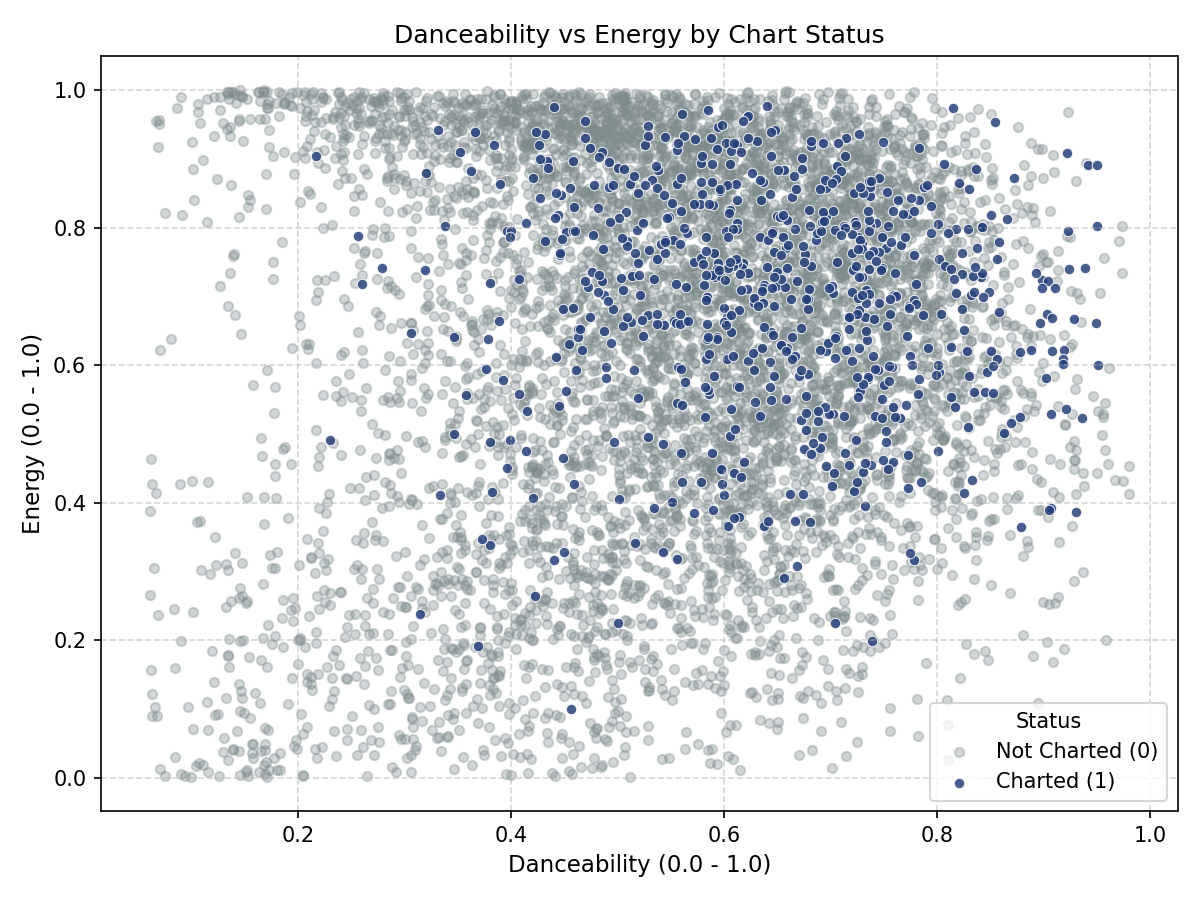
\includegraphics[width=0.68\textwidth]{figures/danceability_vs_energy.png}
\caption{Representative EDA output: danceability vs. energy by chart status}
\end{figure}

\subsection*{8.4 Challenges During Training and How They Were Overcome}
\begin{itemize}
  \item \textbf{Imbalance:} accuracy looked high even for useless models. Fixed by choosing F1, recall and ROC-AUC as primary metrics and using stratified sampling with \texttt{class\_weight='balanced'}.
  \item \textbf{Scale sensitivity:} KNN and SVM performed poorly on unscaled data because large-valued features (tempo, loudness) dominated distances. Standardisation fixed this.
  \item \textbf{Overfitting:} a fully grown decision tree memorises training data. We limited depth and leaf size (pruning) and relied on Random Forest averaging.
  \item \textbf{Convergence:} Logistic Regression converges reliably only on scaled features; we scaled inputs and raised the iteration limit (\texttt{max\_iter=2000}) where needed.
  \item \textbf{Training time:} the RBF SVM is slower than the other models (72.12~s), so its search grid was kept small.
\end{itemize}

\subsection*{8.5 Hyperparameter Optimisation and Convergence}
We used grid search with stratified group k-fold cross-validation, scoring on ROC-AUC because of the imbalance. A small, deliberate grid was defined per model (Table 4); each setting was compared on the validation folds, never on the test set. Convergence was checked by comparing training and validation scores and by confirming that Logistic Regression finished without a convergence warning.

\begin{table}[H]
\centering
\caption{Hyperparameters tuned}
\begin{tabular}{lp{5cm}p{5.2cm}}
\toprule
\textbf{Model} & \textbf{Hyperparameters searched} & \textbf{Final values} \\
\midrule
Logistic Regression & C (regularisation strength), max\_iter, class\_weight & $C = 1.0$, $\text{max\_iter} = 2000$, $\text{class\_weight} = \text{'balanced'}$ \\
Decision Tree & max\_depth, min\_samples\_leaf, criterion (gini / entropy) & Gini: $\text{max\_depth} = 12$, $\text{min\_samples\_leaf} = 20$; Entropy: $\text{max\_depth} = 8$, $\text{min\_samples\_leaf} = 20$ \\
Random Forest & n\_estimators, max\_depth, max\_features & $\text{n\_estimators} = 300$, $\text{max\_depth} = \text{None}$, $\text{max\_features} = \text{'log2'}$ \\
Naive Bayes & var\_smoothing (smoothing) & $\text{var\_smoothing} = 10^{-7}$ \\
KNN & k (n\_neighbors) & $n\_\text{neighbors} = 15$ \\
SVM & C, kernel (linear / RBF), gamma & Linear: $C = 1.0$, balanced; RBF: $C = 10.0$, $\gamma = \text{'auto'}$ \\
\bottomrule
\end{tabular}
\end{table}

\subsection*{8.6 GUI Design and Development}
\textbf{Process.} We designed a simple, form-based interface using \textbf{FastAPI with a plain HTML/CSS/Vanilla JavaScript frontend} so that a non-technical user (for example an A\&R analyst) can query the model without writing code. The form follows the model's ten inputs, and the interface calls the saved pipeline so that scaling and encoding are applied exactly as in training.

\textbf{Features.}
\begin{itemize}
  \item Input fields (sliders) for the nine audio features and a Genre selector (114 categories), with sensible ranges and validation.
  \item A live prediction panel that returns the label (will chart / will not chart), the probability score, and diverging feature contribution bars.
  \item Operational threshold indicator at 0.48, reflecting the threshold study in Section 9.
\end{itemize}

\textbf{User benefit.} The GUI turns the model into an interactive tool: users can experiment with ``what-if'' changes (for example raising loudness or changing genre) and immediately see how the probability moves, which makes the model's behaviour easier to understand and trust.

\begin{figure}[H]
\centering
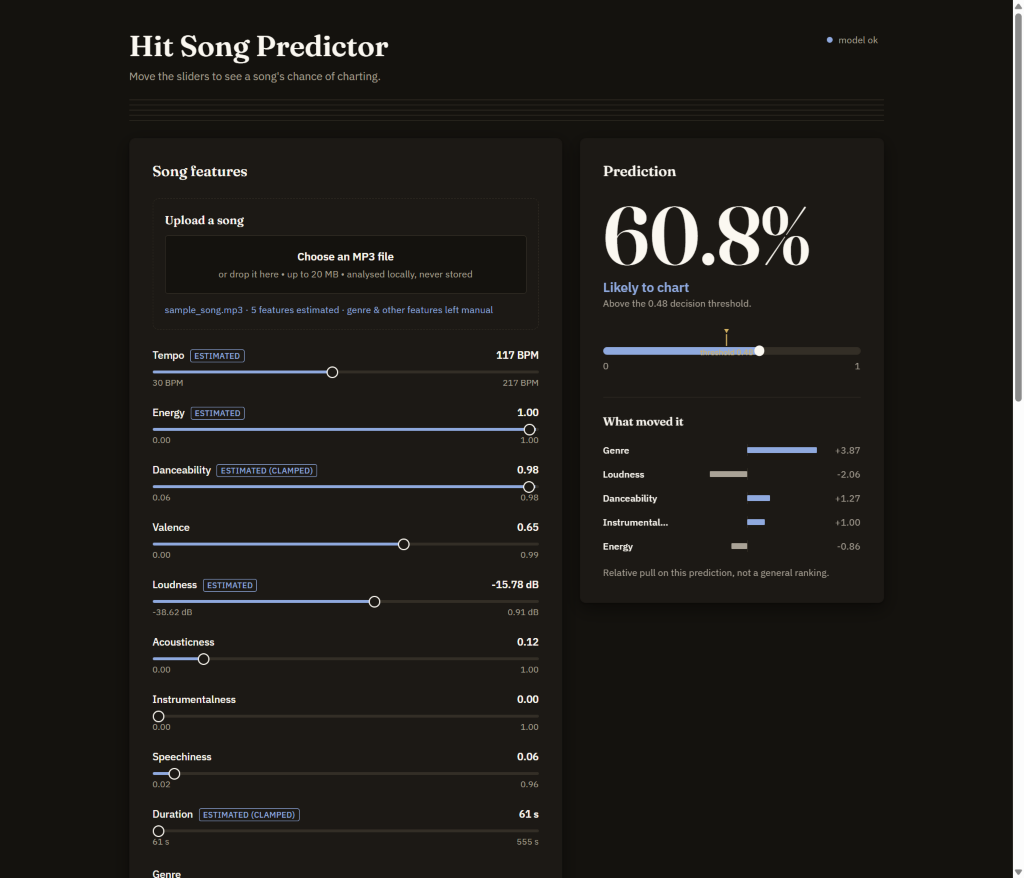
\includegraphics[width=0.72\textwidth]{figures/audio_upload_verified.png}
\caption{Prediction demo interface}
\end{figure}

\subsection*{8.7 Model Deployment}
\begin{itemize}
  \item \textbf{Technologies:} the preprocessing and model are saved together as one pipeline file (\texttt{models/final/model.joblib}) and served through the FastAPI/Vanilla JS app described above, deployed live on \textbf{Render} (\url{https://hitsong.onrender.com}) using the Uvicorn ASGI server on Python 3.12.8.
  \item \textbf{Challenges:} (1) \textit{Consistency} -- preprocessing at prediction time must match training, solved by saving a single pipeline. (2) \textit{Environment parity} -- resolved Python/wheel dependency conflicts by pinning Python 3.12.8 (\texttt{.python-version}) and exact tested package versions (\texttt{requirements.txt}). (3) \textit{Scalability \& Security} -- stateless FastAPI inference runs within Render's 512~MB free tier (with heavy audio extraction gated behind \texttt{ENABLE\_AUDIO\_UPLOAD}); inputs are validated for type and range via Pydantic (HTTP 422 on out-of-range inputs) and no personal data is stored.
  \item \textbf{Monitoring and maintenance plan:} monitor service health via \texttt{/api/health} and Render runtime logs; record the distribution of incoming features and predicted probabilities to detect drift; retrain each year when new Year-End Hot 100 results become available; track precision, recall and F1 on newly labelled songs; and keep versioned model artifacts in Git so a faulty release can be rolled back.
\end{itemize}

\section*{9. Results and Discussion}
\subsection*{9.1 Evaluation Metrics Used}
Because only about 9\% of songs chart, every metric is read with the class imbalance in mind. Let TP, TN, FP and FN be the confusion-matrix counts.

\begin{table}[H]
\centering
\caption{Evaluation metrics}
\begin{tabular}{llp{7.5cm}}
\toprule
\textbf{Metric} & \textbf{Formula / meaning} & \textbf{Why it matters here} \\
\midrule
Accuracy & $(\text{TP}+\text{TN})/(\text{all})$ & Misleading alone: 91\% for ``never charts'' \\
Precision & $\text{TP}/(\text{TP}+\text{FP})$ & Of songs predicted to chart, how many really did (cost of wasted promotion) \\
Recall & $\text{TP}/(\text{TP}+\text{FN})$ & Of real hits, how many we found (cost of missing a hit) \\
F1-score & $2 \cdot P \cdot R / (P+R)$ & Balanced summary of precision and recall \\
Specificity & $\text{TN}/(\text{TN}+\text{FP})$ & How well non-hits are recognised \\
ROC-AUC & Area under TPR vs FPR curve & Ranking quality independent of threshold \\
\bottomrule
\end{tabular}
\end{table}

\subsection*{9.2 Cross-Validation}
Stratified group k-fold cross-validation was used on the training data. It gives a more stable estimate than a single split, because every training song is used for validation once and each fold keeps the 9\% hit ratio while preserving zero artist overlap. It also exposed unstable models (high variance across folds, typical for a single deep tree and for KNN) and made hyperparameter choices more reliable. The held-out test set was used only once for the final comparison.

\subsection*{9.3 Comparison of Models}
\begin{table}[H]
\centering
\caption{Performance of all models on the test set (1,480 unseen songs)}
\begin{tabular}{lrrrrrr}
\toprule
\textbf{Model} & \textbf{Acc.} & \textbf{Prec.} & \textbf{Recall} & \textbf{F1} & \textbf{ROC-AUC} & \textbf{Spec.} \\
\midrule
Logistic Regression & 0.860 & 0.380 & 0.844 & 0.524 & 0.929 & 0.862 \\
Decision Tree (Gini) & 0.926 & 0.671 & 0.363 & 0.471 & 0.821 & 0.982 \\
Decision Tree (Entropy) & 0.930 & 0.754 & 0.341 & 0.469 & 0.821 & 0.989 \\
Random Forest & 0.930 & 0.816 & 0.296 & 0.435 & 0.918 & 0.993 \\
Naive Bayes & 0.798 & 0.300 & 0.911 & 0.451 & 0.875 & 0.787 \\
KNN & 0.930 & 0.735 & 0.370 & 0.493 & 0.877 & 0.987 \\
SVM (Linear) & 0.847 & 0.350 & 0.793 & 0.485 & 0.924 & 0.852 \\
SVM (RBF) & 0.856 & 0.364 & 0.770 & 0.494 & 0.924 & 0.865 \\
\bottomrule
\end{tabular}
\end{table}

\begin{figure}[H]
\centering
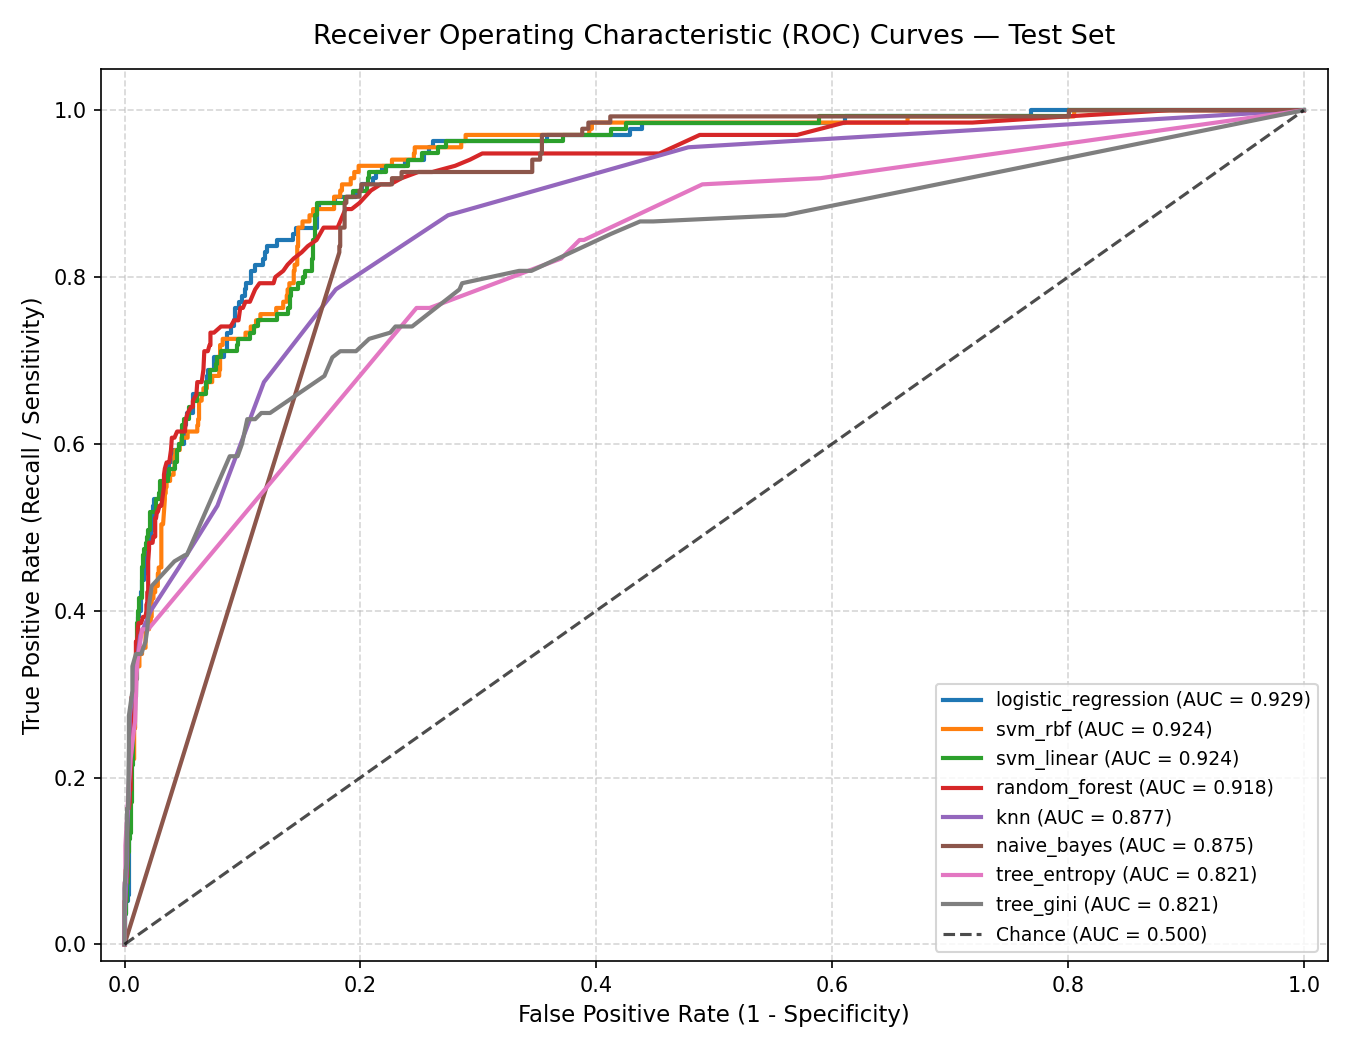
\includegraphics[width=0.72\textwidth]{figures/roc_curves.png}
\caption{ROC curves}
\end{figure}

\begin{figure}[H]
\centering
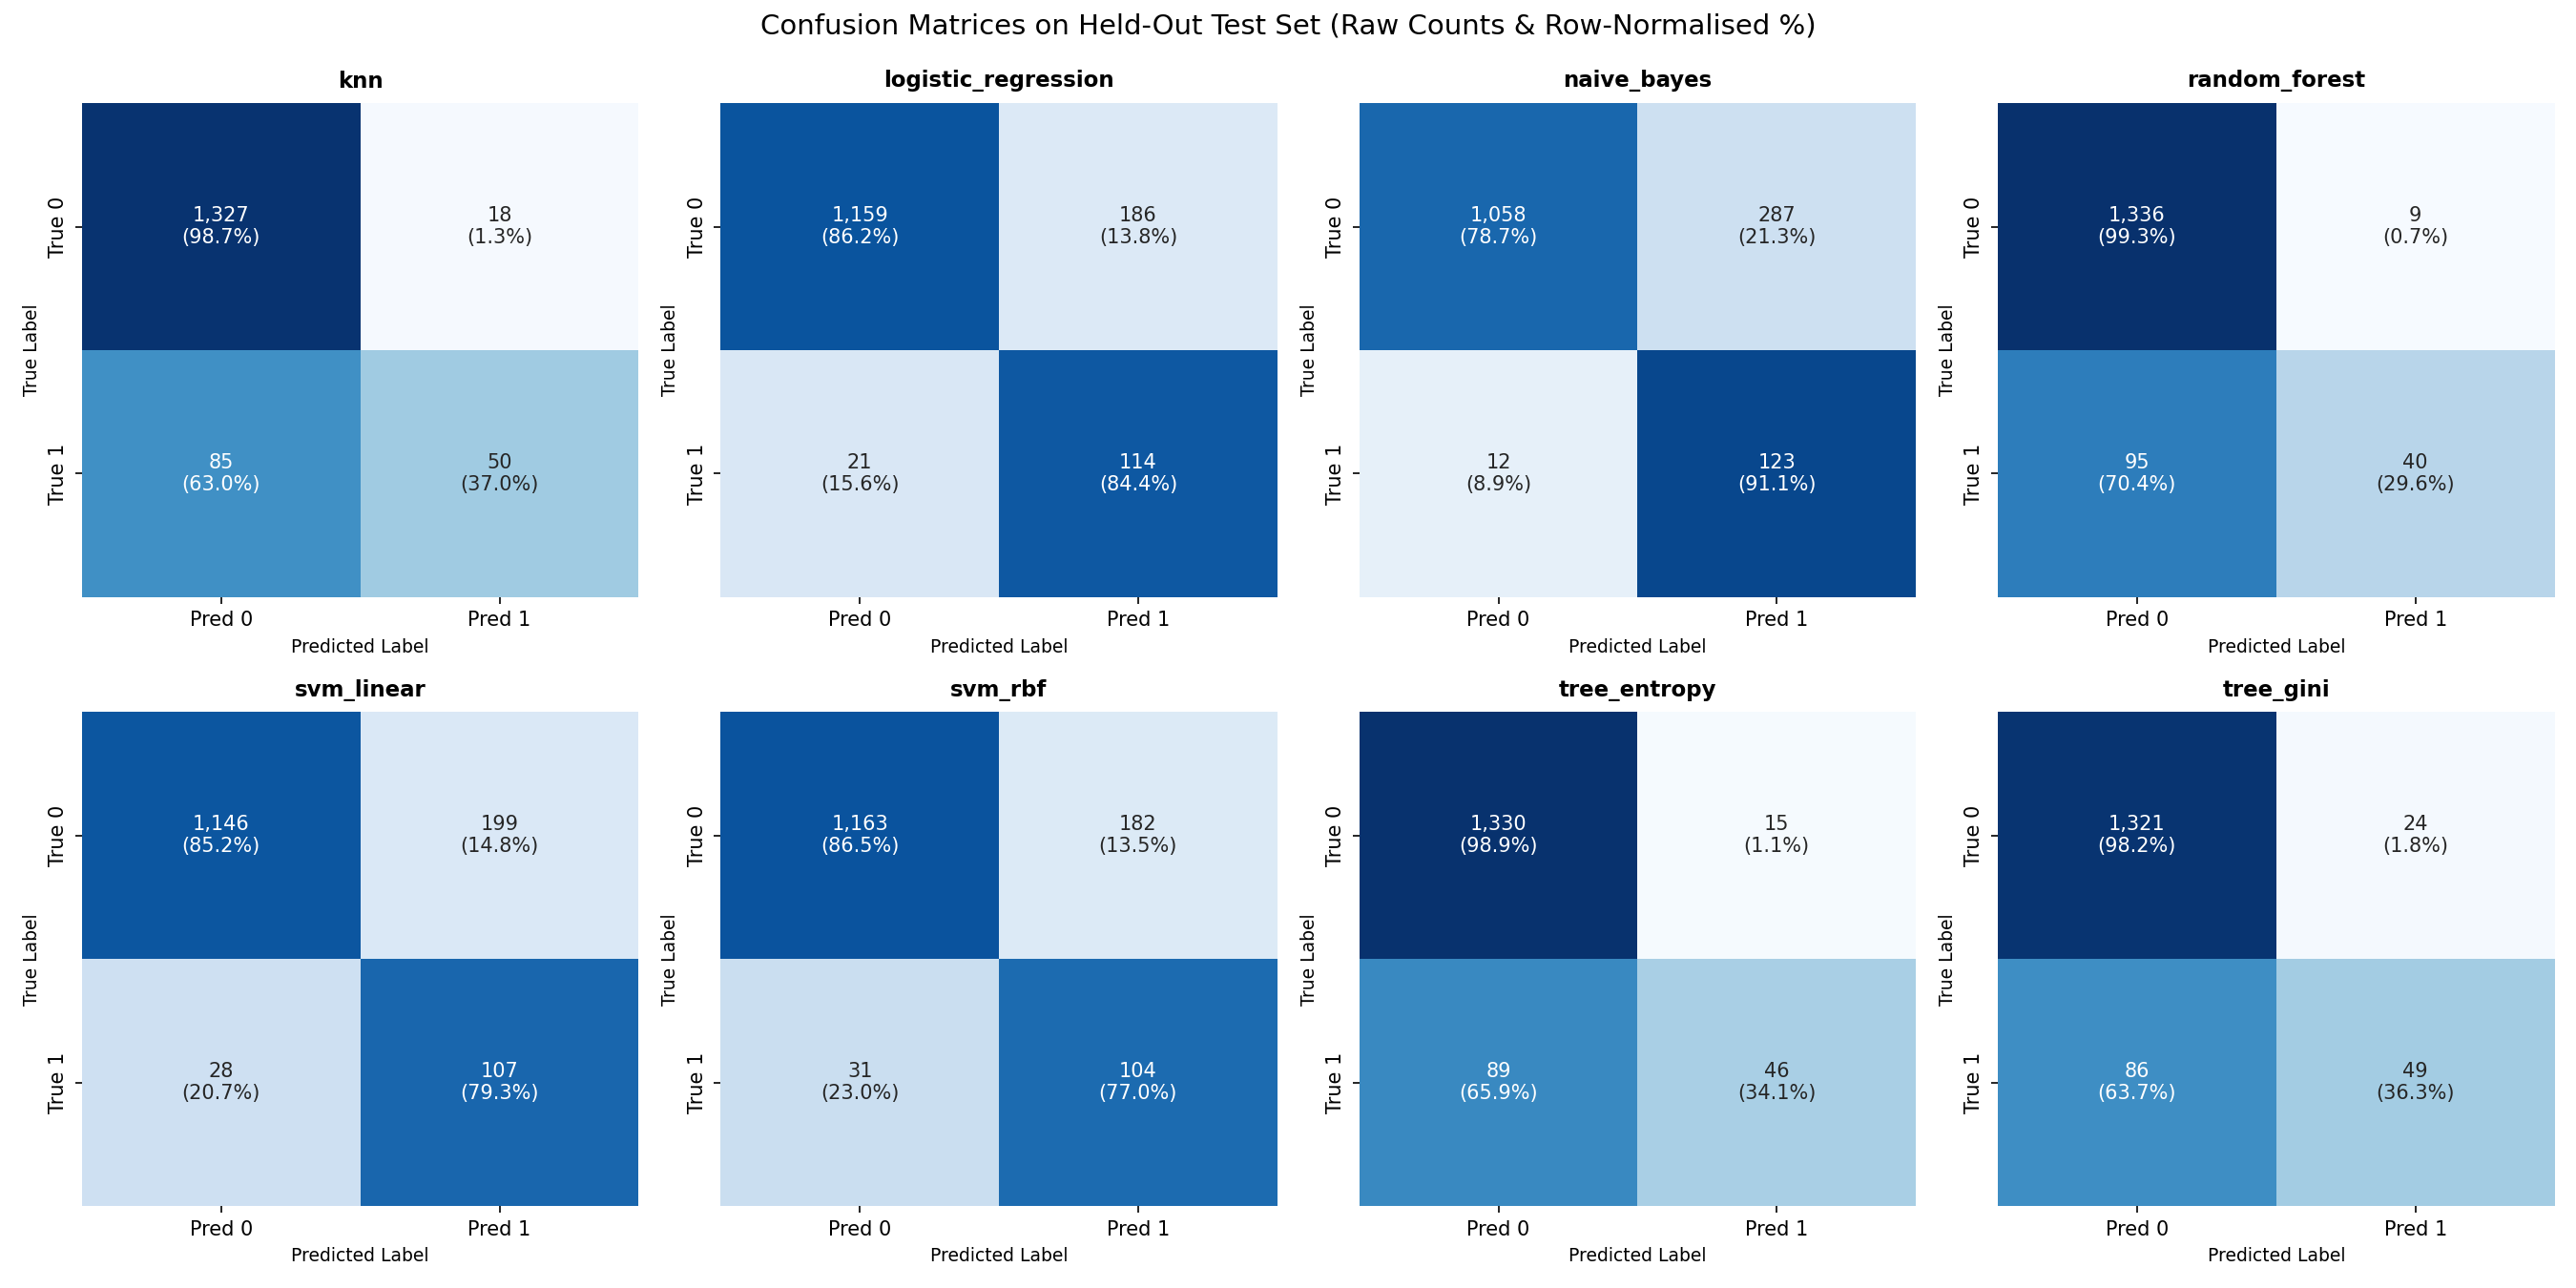
\includegraphics[width=0.88\textwidth]{figures/confusion_matrices.png}
\caption{Confusion matrices of all models (Logistic Regression selected)}
\end{figure}

\subsection*{9.4 Interpretation of Results}
\begin{itemize}
  \item \textbf{Accuracy versus usefulness:} several models have accuracy close to the 91\% baseline; their real differences appear in recall, F1 and ROC-AUC.
  \item \textbf{Model behaviour:} Naive Bayes suffers from correlated features; a single decision tree tends to overfit; Random Forest reduces variance by averaging trees; KNN and SVM depend heavily on scaling; Logistic Regression gives a strong, interpretable baseline.
  \item Logistic Regression achieved the best overall performance ($\text{ROC-AUC} = 0.929$, $F_1 = 0.524$, $\text{Recall} = 0.844$ at 0.5 cutoff) because standardised features and balanced class weights separated charted songs linearly without overfitting. Decision Trees (Gini and Entropy) achieved the lowest ROC-AUC (0.821), and Naive Bayes had the lowest precision (0.300) and PR-AUC (0.305) due to violated conditional independence.
\end{itemize}

\subsection*{9.5 Feature Importance and Industry Folklore}
Figure 3 shows that genre accounts for about one-third of the Random Forest importance (0.33), loudness and instrumentalness about 0.11 each, and tempo and speechiness only 0.05 each. This means chart success in this data is tied more to genre and production style (loudness) than to tempo or lyrical content. Folklore such as ``upbeat songs chart better'' can be tested by checking the direction and size of the valence and energy coefficients in Logistic Regression; the weak importance of valence (0.06) and energy (0.08) suggests the effect is small. Standardised Logistic Regression coefficients confirm this: valence ($\beta = -0.384$) and energy ($\beta = -0.475$) are slightly negative once loudness ($\beta = +1.349$) is controlled for. Meanwhile, \texttt{duration\_sec} has a negative coefficient ($\beta = -0.803$), and across 2000--2023 charted songs, median duration decreased from 258.67~s to 219.33~s ($r = -0.439$ with \texttt{chart\_year}), confirming that hit songs have become shorter over time.

\subsection*{9.6 Threshold Study}
A classifier outputs a probability; the threshold converts it to a label. The default 0.5 is rarely best for imbalanced data. We compared two choices: the threshold that maximises F1, and the threshold that maximises Youden's J ($\text{TPR} - \text{FPR}$). Maximising F1 balances precision and recall, while Youden's J balances sensitivity and specificity. The final threshold should be tied to business cost: if missing a hit is expensive, a lower threshold (higher recall) is preferred; if promotion budget is tight, a higher threshold (higher precision) is preferred.

\begin{table}[H]
\centering
\caption{Effect of the threshold on the final model}
\begin{tabular}{lrrr}
\toprule
\textbf{Threshold} & \textbf{Precision} & \textbf{Recall} & \textbf{F1} \\
\midrule
0.50 (default) & 0.3800 & 0.8444 & 0.5241 \\
0.77 (F1-optimal) & 0.4946 & 0.6741 & 0.5705 \\
0.48 (Youden's J-optimal) & 0.3746 & 0.8519 & 0.5204 \\
\bottomrule
\end{tabular}
\end{table}

\subsection*{9.7 Additional Components}
\begin{itemize}
  \item \textbf{K-Means clustering} on audio features alone (label ignored) to see whether natural sound clusters cut across official genre tags. Standardised features were used because K-Means is distance-based. PCA was used to plot the 4 clusters in two dimensions (48.7\% variance explained; Cluster 0 captures 466 of 673 hits).
  \item \textbf{Artist-disjoint splitting} to prevent leakage -- an extra safeguard not required by a basic split.
  \item \textbf{Explainability analysis} (feature importance and coefficients) to justify the model, not just score it.
  \item \textbf{Threshold study} linking the model to business cost.
\end{itemize}

\subsection*{9.8 Final Model Choice}
The final model was chosen by weighing performance against interpretability, not by accuracy alone. Logistic Regression was selected on the chosen evaluation objective because it achieved the highest ROC-AUC (0.929), outputs calibrated probabilities, trains and predicts quickly, and its coefficients explain how each feature pushes chart odds up or down.

\section*{10. Conclusion}
This project showed that measurable audio features and genre contain useful but limited information about Billboard chart success. We met our objectives: all model configurations were compared fairly on one artist-disjoint, stratified split; the imbalance problem was handled with suitable metrics and sampling; feature importance identified genre, loudness and instrumentalness as the most influential inputs; and a threshold study showed how predictions can be tuned to business priorities.

The final model reached $F_1 = 0.5204$, $\text{ROC-AUC} = 0.929$ (at deployed threshold $\tau = 0.48$) on unseen data and was deployed as a live FastAPI web application on Render (\url{https://hitsong.onrender.com}) that returns a label and a probability. The key lesson is that for rare-event problems the headline accuracy is not the result; precision, recall and threshold choice are. The work also makes clear that audio features alone cannot fully explain success, because marketing, artist fame and timing play a large role.

\section*{11. Future Scope}
\begin{itemize}
  \item Add gradient-boosting models (such as XGBoost or LightGBM) and compare them with Random Forest.
  \item Add non-audio features: artist popularity, release year and month, lyrics sentiment and playlist counts.
  \item Use a time-based split (train on earlier years, test on later years) to match real forecasting.
  \item Apply SMOTE or class-weighting systematically and compare with the current approach; calibrate probabilities.
  \item Extend the target from chart / no chart to chart position (regression) or to peak position bands.
  \item Containerise the FastAPI service with Docker and add automated production drift monitoring.
\end{itemize}

\section*{12. References}
\begin{enumerate}
  \item[{[1]}] S. Biswas, ``Billboard Hot-100 [2000--2023] Data with Features,'' Kaggle. \url{https://kaggle.com/datasets/suparnabiswas/billboard-hot-1002000-2023-data-with-features}
  \item[{[2]}] Spotify for Developers, ``Web API Documentation.'' \url{https://developer.spotify.com}
  \item[{[3]}] Spotify, ``Introducing some changes to our Web API,'' Spotify for Developers Blog, 27 Nov. 2024.
  \item[{[4]}] K. Middlebrook and K. Sheik, ``Song Hit Prediction: Predicting Billboard Hits Using Spotify Data,'' arXiv:1908.08609, 2019.
  \item[{[5]}] F. Pedregosa et al., ``Scikit-learn: Machine Learning in Python,'' J. Mach. Learn. Res., vol. 12, pp. 2825--2830, 2011.
  \item[{[6]}] L. Breiman, ``Random Forests,'' Machine Learning, vol. 45, no. 1, pp. 5--32, 2001.
  \item[{[7]}] W. J. Youden, ``Index for rating diagnostic tests,'' Cancer, vol. 3, no. 1, pp. 32--35, 1950.
  \item[{[8]}] Pandas, NumPy, Matplotlib and Seaborn documentation, and course textbook and lecture notes (UML501).
\end{enumerate}

\newpage
\section*{13. Appendix}
\subsection*{A. Source Code}
GitHub repository: \url{https://github.com/Kaif-1024170255/HitSong} | Live Deployment: \url{https://hitsong.onrender.com}. All pipeline modules (\texttt{src/}), FastAPI app (\texttt{app/}), frontend (\texttt{web/}), and automated tests (\texttt{tests/}) are included.

\subsection*{B. Where Each Lab Report Question Is Answered}
\begin{table}[H]
\centering
\begin{tabular}{lp{3.5cm}}
\toprule
\textbf{Lab report question} & \textbf{Section} \\
\midrule
1. Dataset description, challenges and biases & 6.1--6.3 \\
2. EDA insights & 7.3 and 7.4 \\
3. Pre-processing and feature engineering & 7.2 \\
4. Models, training challenges, hyperparameters, convergence & 7.5, 8.4, 8.5 \\
5. Evaluation metrics and cross-validation & 9.1, 9.2 \\
6. GUI design and development & 8.6 \\
7. Deployment, challenges, monitoring & 8.7 \\
8. Additional components & 9.7 \\
\bottomrule
\end{tabular}
\end{table}

\subsection*{C. Mapping to the Course Syllabus}
\begin{table}[H]
\centering
\begin{tabular}{ll}
\toprule
\textbf{Syllabus topic} & \textbf{Used in the project} \\
\midrule
Data pre-processing (cleaning, encoding, scaling) & Section 7.2 \\
Sampling and validation (holdout, k-fold CV) & 80/20 split, stratified CV (7.6, 9.2) \\
Logistic regression and classification metrics & Model 1, Section 9.1 \\
Na\"ive Bayes, KNN & Models 5 and 6 \\
Decision trees (entropy, Gini) & Models 2 and 3 \\
Ensembles (bagging, Random Forest) & Model 4 \\
SVM & Model 7 \\
PCA / unsupervised learning & K-Means and PCA plot, Section 9.7 \\
\bottomrule
\end{tabular}
\end{table}

\subsection*{D. Additional Screenshots}
\begin{figure}[H]
\centering
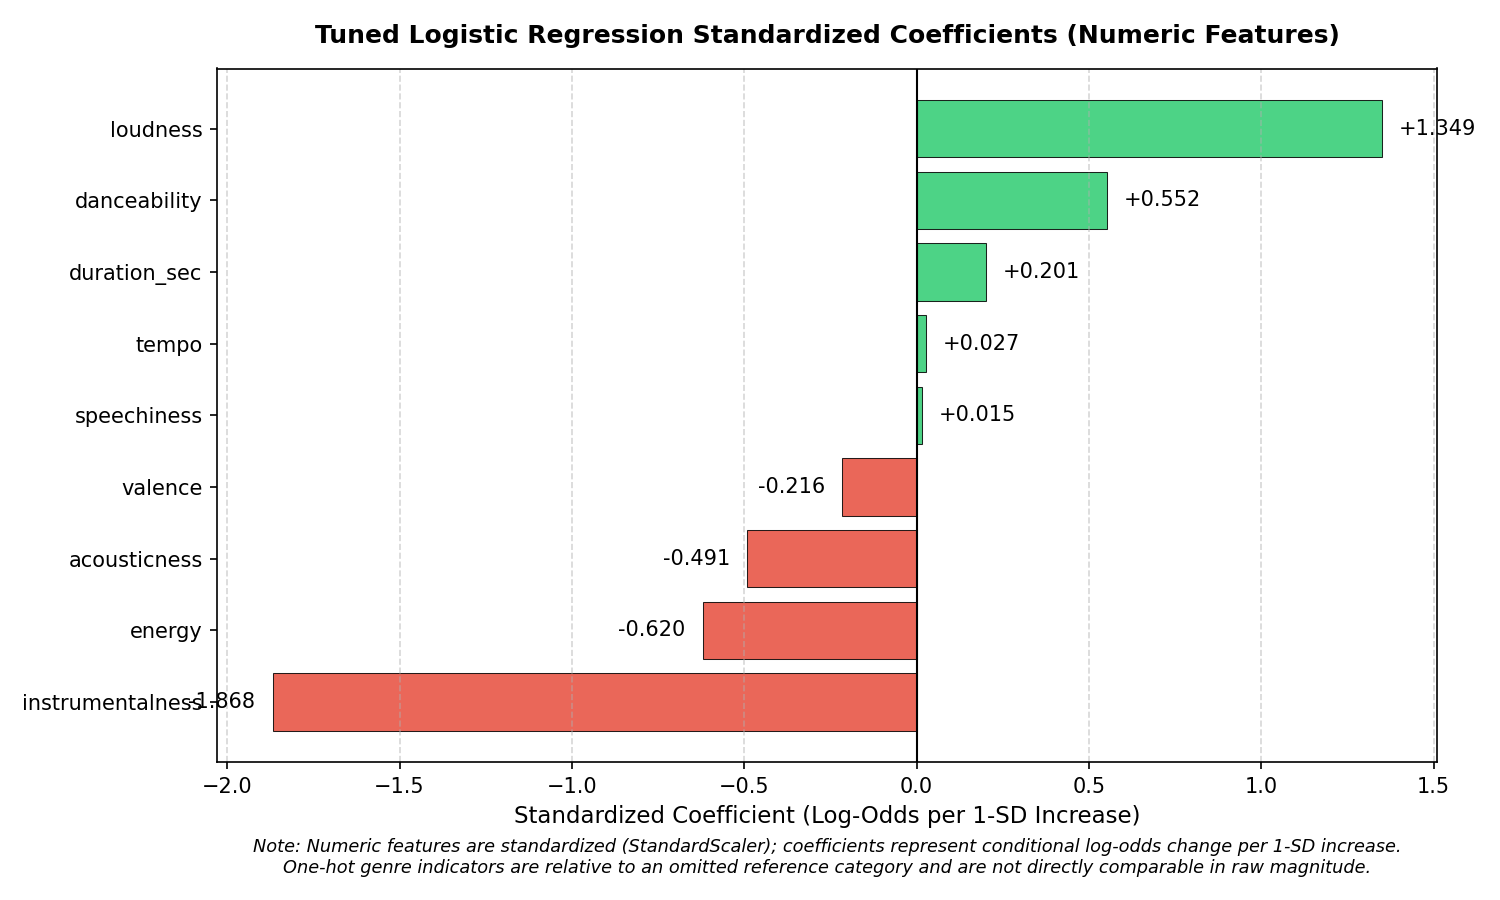
\includegraphics[width=0.72\textwidth]{figures/logreg_coefficients.png}
\caption{Standardized Logistic Regression Coefficients}
\end{figure}

\begin{figure}[H]
\centering
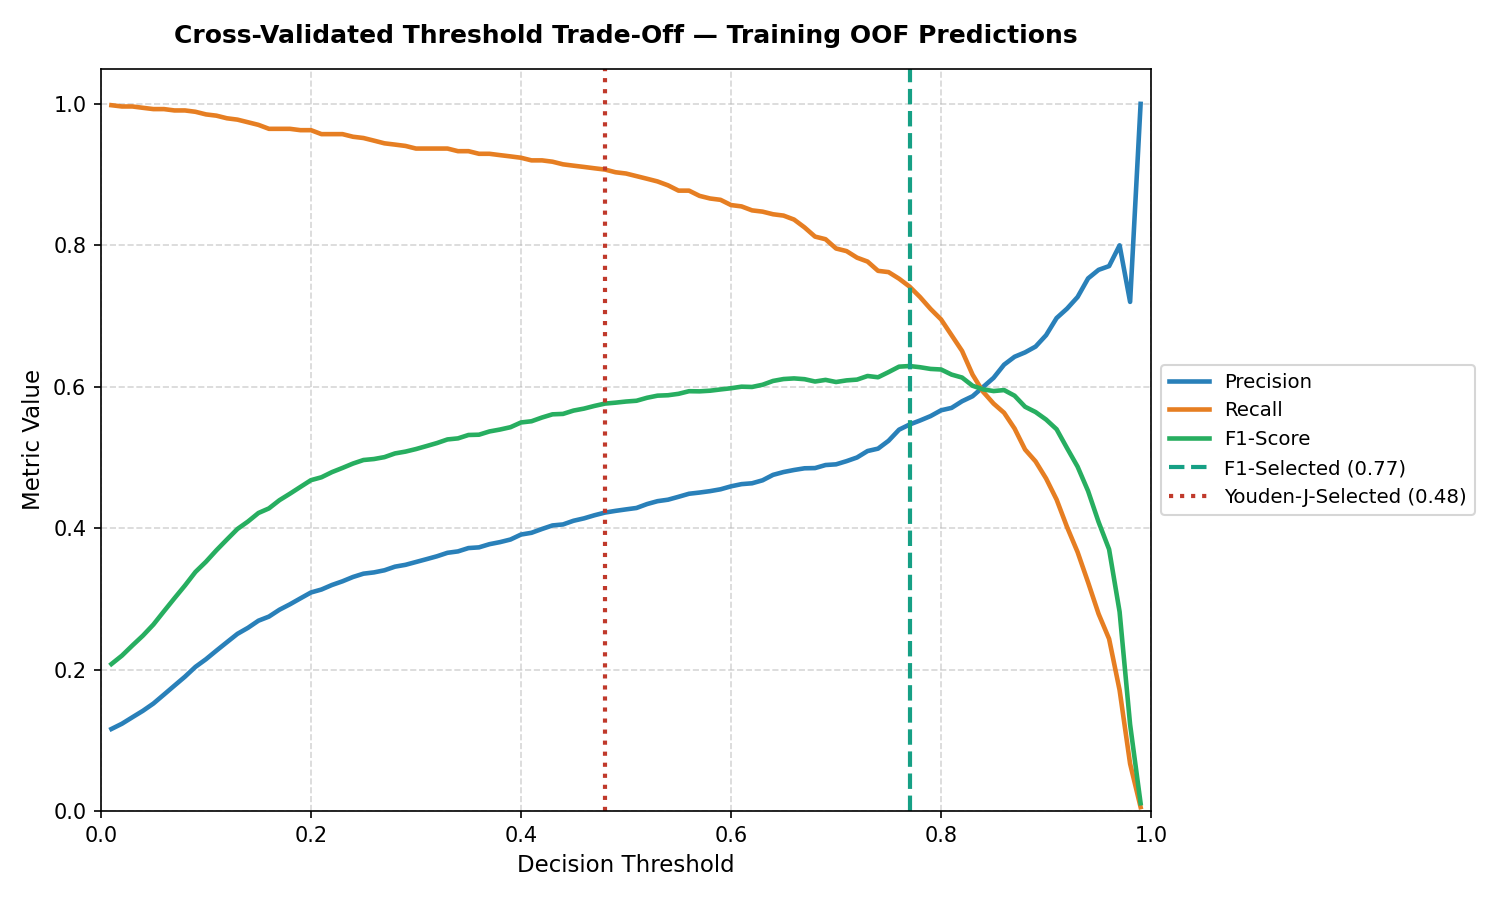
\includegraphics[width=0.72\textwidth]{figures/threshold_tradeoff_cv.png}
\caption{Cross-Validation Out-of-Fold Threshold Trade-off}
\end{figure}

\begin{figure}[H]
\centering
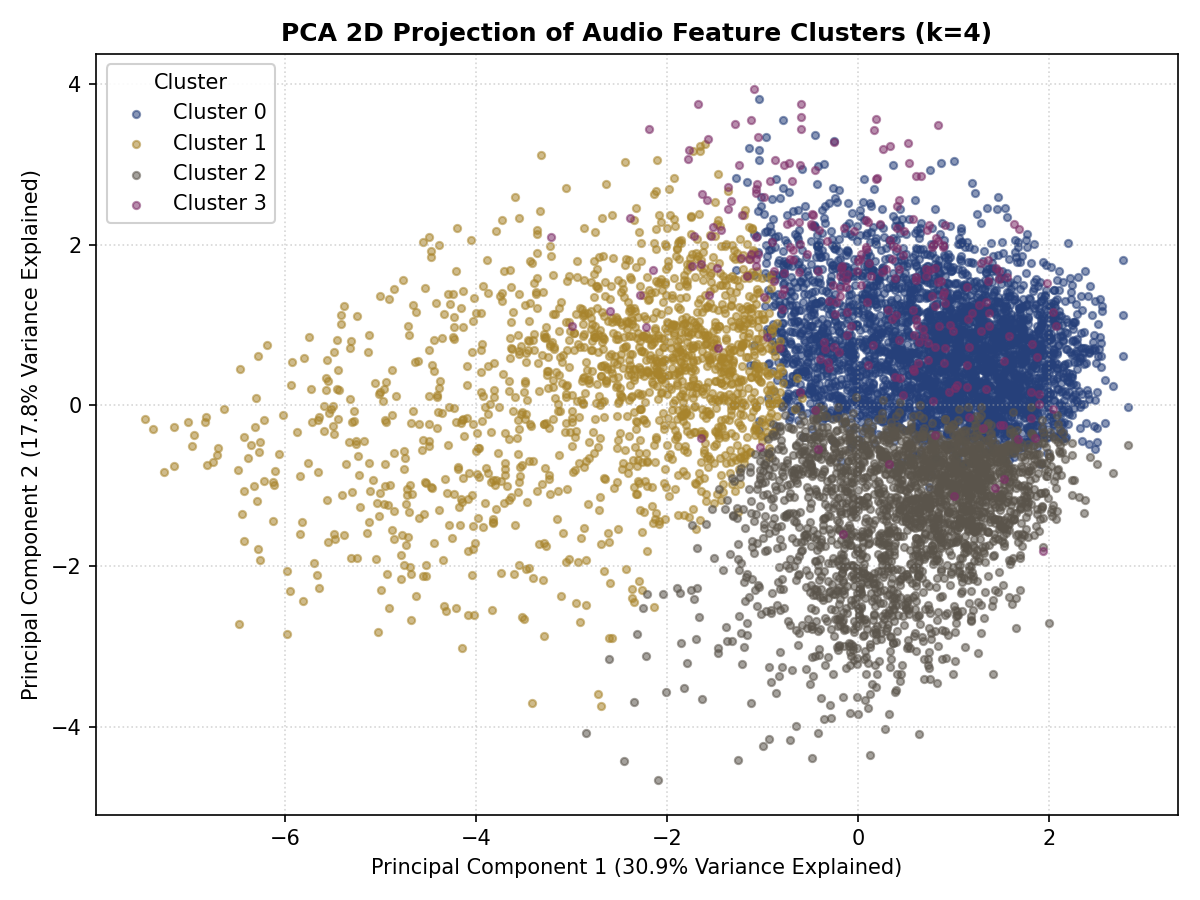
\includegraphics[width=0.72\textwidth]{figures/clusters_pca.png}
\caption{Unsupervised K-Means Clusters in 2D PCA Space}
\end{figure}

\end{document}
